\documentclass[10pt]{beamer}
\usepackage{ragged2e} % \justifying
\usepackage{bm}
\usepackage{tensor}
\newcommand\norm[1]{\left\lVert#1\right\rVert}
\newcommand{\at}[2][]{#1|_{#2}}
\usetheme{metropolis}           % Use metropolis theme
\title{FP2: Torso Pose Estimation on the \\HRP4 Humanoid Robot}
\subtitle{Michele Cipriano, Godwin K. Peprah, Lorenzo Vianello}
\date{}
\author{\textit{Supervisor:} Nicola Scianca\\
    \textit{Professors:} Giuseppe Oriolo, Alessandro De Luca\\}
\institute{Autonomous and Mobile Robotics, Robotics 2\\
    Department of Computer, Control and Management
    Engineering\\Sapienza University of Rome}

% Fontsize of figure smaller than normalsize:
\setbeamerfont{caption}{size=\scriptsize}

\begin{document}
\nocite{*}

    \maketitle

    \begin{frame}{Introduction}
        \begin{itemize}
            \item Aim of the project following methodology in [1]
            \item Pose of the torso for localization of robot points using encoder readings.
            \item Estimate used to close feedback loop in the MPC gait generator
            \item Estimation done with EKF using standard humanoid sensors
            \item Use of accelerometer and the gyroscope of the IMU and improving results with a filter
            \item Trilateration algorithm used as last step
            \item Testing the behaviour of the EKF through regulation tasks
            \item C++ and HRP4 robot model in a V-REP environment used
        \end{itemize}
    \end{frame}

    \begin{frame}{Kinematic Model}
        \justifying
%        Let $\bm{x} = (\bm{p}_t^T, \bm{o}_t^T)^T$ be the pose of $\mathcal{F}_t$
%        wrt $\mathcal{F}_w$. %We want to
        %develop a filter that estimates the state $\bm{x}$ while
        %it moves around the environment.
%        Let $\mathcal{F}_s$ be the
%        support foot frame with respect to the world frame and let
%        $\bm{o}_s$ be its orientation.
%        Let $\bm{J}(\bm{q}_s, \bm{o}_s)$ the Jacobian
%        matrix of the kinematic map from the support frame
%        $\mathcal{F}_s$ to the torso frame $\mathcal{F}_t$.

        Let's use the following kinematic model to describe the
        evolution of the state $\bm{x}$ through time:
        \begin{equation*}
            \bm{\dot{x}} = \bm{J}(\bm{q}_s, \bm{o}_s) \bm{\dot{q}}_s
        \end{equation*}
        with $\bm{o}_s$ orientation of $\mathcal{F}_s$ and
        $\bm{\dot{q}}_s$ velocities of the support joints
        acting as control inputs.
%        Note that the Jacobian
%        $\bm{J}(\bm{q}_{s}, \bm{o}_s)$ does not depend on the
%        position of $\mathcal{F}_s$:
%        \begin{align*}
%            \bm{f}(\bm{q}_s, \bm{o}_s) %&= \bm{\varOmega} \left(
                %\begin{bmatrix}
                %    \bm{R}_z(\bm{o}_s) & \bm{0} \\
                %    \bm{0}^T & 1
                %\end{bmatrix}
                %\bm{\varOmega}^{-1}\left(
                %\begin{bmatrix}
                %     \tensor[^s]{\bm{p}}{_t} \\
                %     \tensor[^s]{\bm{o}}{_t}
                %\end{bmatrix}
                %\right)
                %\right) \\
                %&= \bm{\varOmega} \left(
                %\begin{bmatrix}
                %    \bm{R}_z(\bm{o}_s + \tensor[^s]{\bm{o}}{_{t,z}}) \bm{R}_y(\tensor[^s]{\bm{o}}{_{t,y}}) \bm{R}_x(\tensor[^s]{\bm{o}}{_{t,x}}) & \bm{R}_z(\bm{o}_s) \tensor[^s]{\bm{p}}{_t}  \\
                %    \bm{0}^T & 1
                %\end{bmatrix}
                %\right) \numberthis \\
%                &=
%                \begin{bmatrix}
%                    \bm{R}_z(\bm{o}_s) & \bm{O} \\
%                    \bm{O} & \bm{I}
%                \end{bmatrix}
%                \bm{f}(\bm{q}_s)
%                +
%                \begin{pmatrix}
%                    \bm{0}_{5} \\
%                    \bm{o}_s
%                \end{pmatrix} \\
%            \bm{J}(\bm{q}_s, \bm{o}_s) %&= \frac{\partial \bm{f}(\bm{q}_s, \bm{o}_s)}{\partial \bm{q}_s} \\
            %&=
            %\begin{bmatrix}
            %        \bm{R}_z(\bm{o}_s) & \bm{O} \\
            %        \bm{O} & \bm{I}
            %\end{bmatrix}
            %\frac{\partial \bm{f}(\bm{q}_s)}{\partial \bm{q}_s} \numberthis \\
%            &=
%            \begin{bmatrix}
%                    \bm{R}_z(\bm{o}_s) & \bm{O} \\
%                    \bm{O} & \bm{I}
%            \end{bmatrix}
%            \bm{J}(\bm{q}_s)
%        \end{align*}

        The robot is equipped with a RGBD camera and an IMU, used
        to measure the pose of the torso frame:
        \begin{equation*}
            \bm{y} = \bm{h}(\bm{x}, \bm{q}_n) =
                \begin{pmatrix}
                    \bm{p}_t \\
                    \bm{o}_t
                \end{pmatrix}
        \end{equation*}
    \end{frame}

    \begin{frame}{Extended Kalman Filter}
        \justifying
        It is now possible to define a discrete-time stochastic system:
        \begin{align*}
            \bm{x}_{k+1} &= \bm{x}_k + T \bm{J}(\bm{q}_{s,k}, \bm{o}_s) \bm{\dot{q}}_{s,k} + \bm{v}_k \\
            \bm{y}_k &= \bm{h}(\bm{x}_k, \bm{q}_{n,k}) + \bm{w}_k
        \end{align*}
        %with $k$ current timestep, $T$ sampling interval,
        with
        $\bm{v}_k \sim \bm{\mathcal{N}}(\bm{0}, \bm{V}_k)$ and
        $\bm{w}_k \sim \bm{\mathcal{N}}(\bm{0}, \bm{W}_k)$ zero-mean
        white Gaussian noises and
        $\bm{V}_k \in \mathbb{R}^{6 \times 6}$,
        $\bm{W}_k \in \mathbb{R}^{6 \times 6}$ their respective
        covariance matrices.
    \end{frame}

    \begin{frame}{Extended Kalman Filter: Prediction}
        %%% EKF Prediction.
        \justifying
        At each timestep $k$, a prediction $\bm{\hat{x}}_{k+1|k}$ is
        generated using %the current estimate
        $\bm{\hat{x}}_{k}$:
        \begin{equation*}
            \bm{\hat{x}}_{k+1|k} = \bm{\hat{x}}_k + \bm{J}(\bm{q}_{s,k}, \bm{o}_s) \Delta \bm{q}_{s,k},
            \quad \Delta \bm{q}_{s,k} = \bm{q}_{s,k+1} - \bm{q}_{s,k}
        \end{equation*}
        with $\Delta \bm{q}_{s,k} \approx T \bm{\dot{q}}_{s,k}$
        obtained using encoder readings. \\The covariance prediction
        matrix is updated accordingly:
        \begin{equation*}
            \bm{P}_{k+1|k} = \bm{P}_{k} + \bm{V}_{k}
        \end{equation*}
        The predicted output
        associated to $\bm{\hat{x}}_{k+1|k}$ is computed as well:
        \begin{equation*}
            \bm{\hat{y}}_{k+1|k} = \bm{h}(\bm{\hat{x}}_{k+1|k}, \bm{q}_{n, k+1})
        \end{equation*}
    \end{frame}

    \begin{frame}{Extended Kalman Filter: Correction}
        %%% EKF Correction.
        \justifying
        It is possible to determine the corrected state estimate by computing:
        \begin{equation*}
            \bm{\hat{x}}_{k+1} = \bm{\hat{x}}_{k+1|k} + \bm{G}_{k+1} \bm{\nu}_{k+1}
        \end{equation*}
        with $\bm{\nu}_{k+1} = \bm{y}_{k+1} - \bm{\hat{y}}_{k+1|k}$ innovation
        and $\bm{G}_{k+1}$ Kalman gain matrix:
        \begin{gather*}
            \bm{G}_{k+1} = \bm{P}_{k+1|k} \bm{H}_{k+1}^T \left( \bm{H}_{k+1} \bm{P}_{k+1|k} \bm{H}_{k+1}^T + \bm{W}_{k+1} \right)^{-1} \\
            \bm{H}_{k+1} = \frac{\partial \bm{h}}{\partial \bm{x}} \at[\bigg]{\bm{x}=\bm{\hat{x}}_{k+1|k}}
        \end{gather*}
        The corrected covariance matrix is updated as well:
        \begin{equation*}
            \bm{P}_{k+1} = \bm{P}_{k+1|k} - \bm{G}_{k+1} \bm{H}_{k+1} \bm{P}_{k+1|k}
        \end{equation*}
    \end{frame}

    \begin{frame}{Extended Kalman Filter: Correction}
        Note that, in our implementation, we defined $\bm{V}$ and $\bm{W}$ as:
        \begin{align*}
            \bm{V} &= \text{diag}\{5, 5, 5, 100, 100, 100 \} \cdot 10^{-6} \\
            \bm{W} &= \text{diag}\{5, 5, 5, 5 \cdot 10^{-2}, 5 \cdot 10^{-2}, 5 \cdot 10^{-2} \}  \cdot 10^{-2}
        \end{align*}
    \end{frame}

    \begin{frame}{Accelerometer Integration}
        Considering a constant acceleration $\bm{\ddot{p}}_{t, k}$ in an
        interval $[t_k, t_{k+1})$:
        \begin{align*}
            \bm{\dot{p}}_{t, k+1} &= \bm{\dot{p}}_{t, k} + \bm{\ddot{p}}_{t, k} T \\
            \bm{p}_{t, k+1} &= \bm{p}_{t, k} + \bm{\dot{p}}_{t, k} T + \frac{1}{2} \bm{\ddot{p}}_{t, k} T^2
        \end{align*}
        At each timestep $k$, the accelerometer returns the linear acceleration
        $\tensor[^t]{\bm{a}}{_{t,k}}$ expressed in $\mathcal{F}_t$.
        It must be transformed to $\mathcal{F}_w$:
        \begin{equation*}
            \bm{\ddot{p}}_{t,k} = \tensor[^w]{\bm{R}}{_t}(\bm{\hat{x}}_{k}) \tensor[^t]{\bm{a}}{_{t,k}}
        \end{equation*}
        with:
        \begin{equation*}
            \tensor[^w]{\bm{R}}{_t}(\bm{\hat{x}}_{k}) = \bm{R}_z(\gamma) \bm{R}_y(\beta) \bm{R}_x(\alpha)
        \end{equation*}
        where $\alpha$, $\beta$ and $\gamma$ respectively
        roll, pitch and yaw angles of $\bm{\hat{x}}_{k}$.
    \end{frame}

    \begin{frame}{Gyroscope Integration}
        Considering a constant angular velocity in an interval $[t_k, t_{k+1})$:
        \begin{equation*}
            \bm{o}_{t,k+1} = \bm{o}_{t,k} + T \bm{\dot{o}}_{t,k}
        \end{equation*}
        At each timestep $k$, the gyroscope returns the angular velocity in
        $\tensor[^t]{\bm{\omega}}{_{t,k}}$ expressed in $\mathcal{F}_t$.
        It must be transformed to $\mathcal{F}_w$:
        \begin{equation*}
            \bm{\dot{o}}_{t,k} = \bm{T}(\bm{\hat{x}}_{k}) \tensor[^t]{\bm{\omega}}{_{t,k}}
        \end{equation*}
        with:
        \begin{equation*}
            \bm{T}(\bm{\hat{x}}_{k}) =
            \begin{pmatrix}
                \text{cos}(\gamma)/\text{cos}(\beta) & \text{sin}(\gamma)/\text{cos}(\beta) & 0 \\
                -\text{sin}(\gamma) &  \text{cos}(\gamma) & 0 \\
                \text{cos}(\gamma) \text{tan}(\beta) & \text{sin}(\gamma) \text{tan}(\beta) & 1
            \end{pmatrix}
        \end{equation*}
        where $\beta$ and $\gamma$  respectively
        pitch and yaw angles of $\bm{\hat{x}}_{k}$.
    \end{frame}

    \begin{frame}{EKF with IMU Integration}
        \begin{figure}
        \caption{Experiments (5.1).}
        \centering
        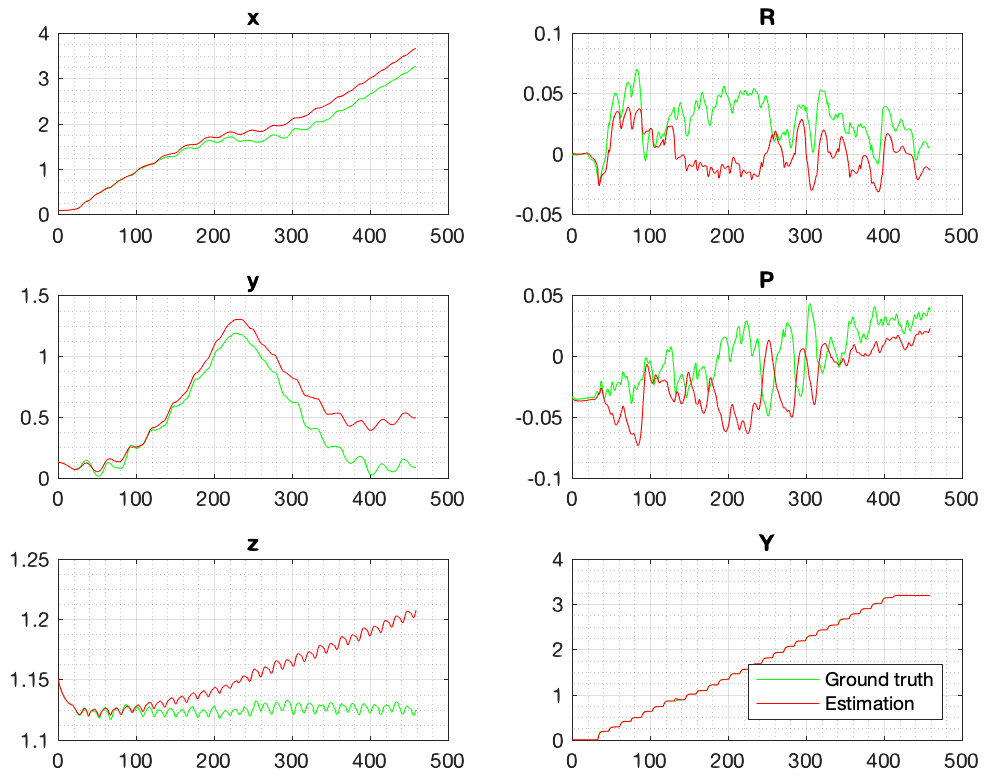
\includegraphics[width=0.75\textwidth]{images/accelerometer.png}
        \end{figure}
    \end{frame}

    \begin{frame}[fragile]{Filtering Linear Velocities}
        Add to the state an approximated estimation of the velocity in such a way to fix drift accumulation.

        Velocity is obtained using position of the robot in 2 successive frames
        \begin{equation*}
            \bm{\dot{p}}_{t,k} \approx \bm{\dot{\hat{p}}}_{t,k} \approx \bm{\dot{\hat{p}}}_{t,k-1}
            = \frac{\bm{\hat{p}}_{t,k} - \bm{\hat{p}}_{t,k-1}}{T}
        \end{equation*}
    \end{frame}

    \begin{frame}[fragile]{Filtering Linear Velocities}
        \begin{figure}
        \caption{Improves the estimate of $(x, y)^{T}$ coordinates decreasing the error on $z$.}
        \centering
        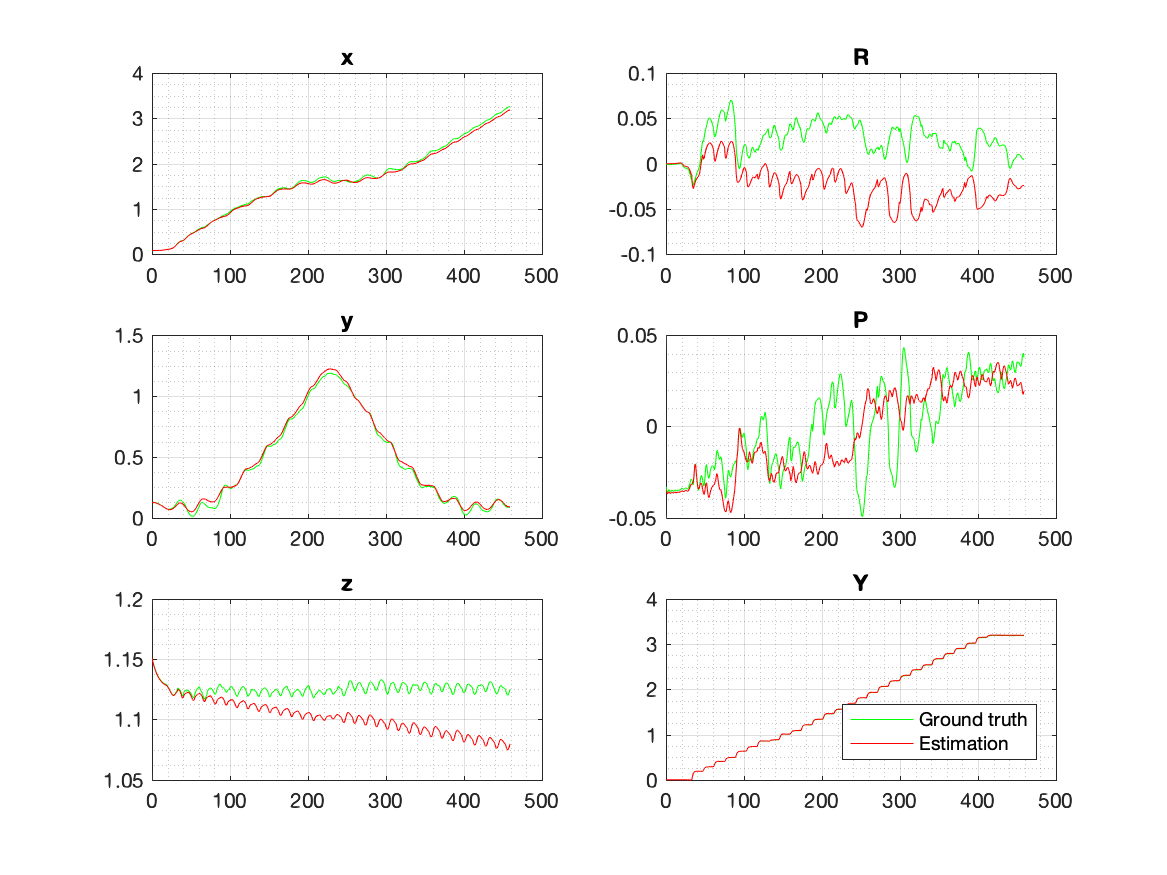
\includegraphics[width=0.75\textwidth]{images/accelerometer_prev_linearvelocity.png}
    \end{figure}

    \end{frame}

    \begin{frame}[fragile]{Trilateration}
        Remove integration and double integration from the calculus of the position.

        Required stuff: RGBD camera posed on the head of the robot, identifiable landmarks with known positions.

        TODO: QUI FORSE CI STA UNO SCREENSHOOT PER MOSTRARE LA CONFIGUARZINE... E FOTO TIPO TRILATERATION
    \end{frame}

    \begin{frame}[fragile]{Trilateration}
        Obtain the distance of the landmarks from the camera:
        \begin{align*}
            ^{cam}{x}{} &= \frac{2 p_x - w}{w} ^{cam}{z}{} \cdot tan\left(\frac{\phi}{2}\right) \\
            ^{cam}{y}{} &= \frac{2 p_y - h}{h} ^{cam}{z}{} \cdot tan\left(\frac{\phi}{2}\right) \\
            ^{cam}{z}{} &= (\lambda_f - \lambda) \cdot p_z + \lambda \\
        \end{align*}
        \begin{equation*}
            r_i =
            \norm{
                \begin{pmatrix}
                    ^{cam}{x}{_i} \\
                    ^{cam}{y}{_i} \\
                    ^{cam}{z}{_i}
                \end{pmatrix}
                }^2 + \bar{r} \quad (i = 1, 2, \dots, n)
        \end{equation*}

        FOTO TIPO CAMERA MODEL
    \end{frame}

    \begin{frame}[fragile]{Trilateration}
        Knowing position of each landmarks in the world frame $(x_{i}, y_{i}, z_{i})^{T}$ and its distance from the camera $r_{i}$, find the position of the camera is equal to resolve an equation for landmark
        \begin{equation*}
            (p_{h,x} - x_i)^2 + (p_{h,y} - y_i)^2 + (p_{h,z} - z_i)^2 = r_i^2 \quad (i = 1, 2, \dots, n)
        \end{equation*}
        which can be rewritten as linear system $Ax= b$:
        \begin{equation*}
        \bm{A} = \begin{pmatrix}
                x_2 - x_1 & y_2 - y_1 & z_2 - z_1 \\
                x_3 - x_1 & y_3 - y_1 & z_3 - z_1 \\
                \vdots & \vdots & \vdots \\
                x_n - x_1 & y_n - y_1 & z_n - z_1
            \end{pmatrix}, \quad
        \bm{x} =
            %\begin{pmatrix}
            %    x - x_1 \\
            %    y - y_1 \\
            %    z - z_1
            %\end{pmatrix}, \quad
            \bm{p}_h -
            \begin{pmatrix}
                x_1 \\
                y_1 \\
                z_1
            \end{pmatrix}, \quad
        \bm{b} = \begin{pmatrix}
                b_{21} \\
                b_{31} \\
                \vdots \\
                b_{n1}
            \end{pmatrix}
    \end{equation*}

    \begin{equation*}
        b_{k1} = \frac{1}{2}\left[ r_1^2 + r_k^2 + (x_k - x_1)^2 + (y_k - y_1)^2 + (z_k - z_1)^2 \right] \quad (k = 2, 3, \dots, n)
    \end{equation*}

    \end{frame}

    \begin{frame}[fragile]{Trilateration}
        Hence, the position of the torso can be determined by:
        \begin{equation*}
            %\begin{pmatrix}
            %    x \\
            %    y \\
            %    z
            %\end{pmatrix}
            \bm{p}_h
                =
            \bm{x} +
            \begin{pmatrix}
                x_1 \\
                y_1 \\
                z_1
            \end{pmatrix} \quad
            \bm{p}_t = \bm{p}_h - \tensor[^w]{\bm{R}}{_t}(\bm{\hat{x}}_{k}) (\tensor[^t]{\bm{p}}{_h} - \tensor[^t]{\bm{p}}{_t})
        \end{equation*}
        We need at least 5 landmarks for the computation: 4 for obtain a
        square matrix, and at least 1 more for execute the pseudoinverse that
        bring results also in case of noisy measurements.
    \end{frame}

    \begin{frame}[fragile]{Trilateration}
        \begin{figure}
        \caption{Improved estimation for $x, y, z$}
        \centering
        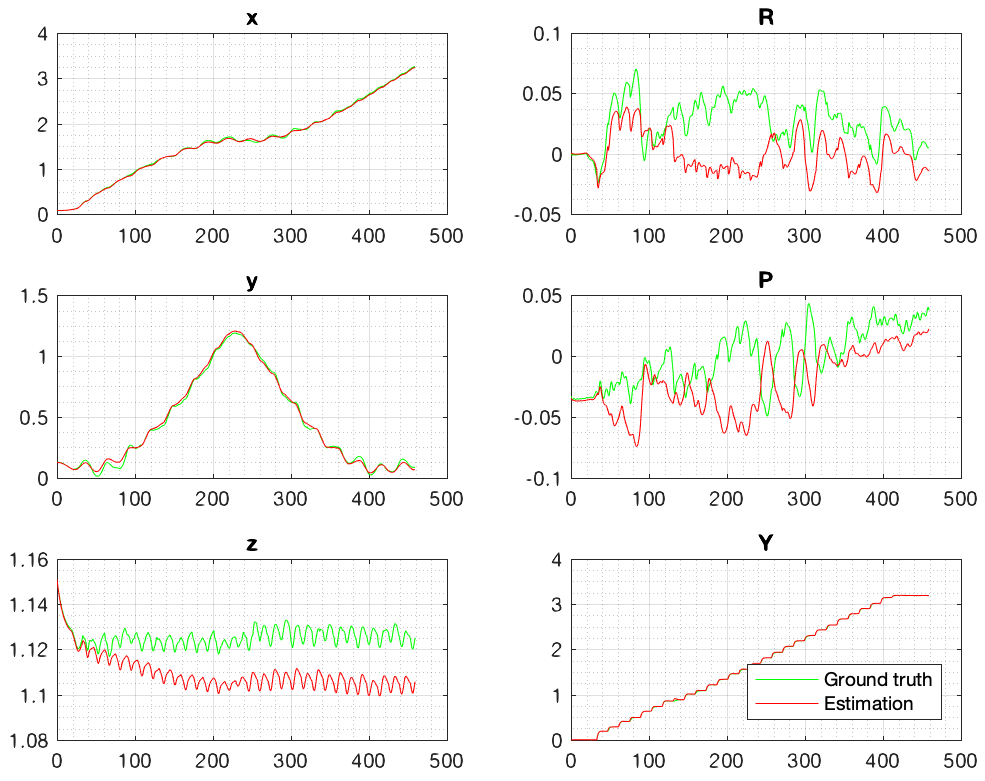
\includegraphics[width=0.75\textwidth]{images/trilateration.png}
        \end{figure}
    \end{frame}

    \section{MPC Loop Closure}

    \begin{frame}{MPC Loop CLosure}
    	The MPC need the position of the CoM with respect to the support
        foot to close the loop.

    	We want to estimate the same position but with the support foot
        reference frame with roll e pitch (wrt world frame) equal to zero.
    \end{frame}

    \begin{frame}{MPC Loop CLosure}
    	\begin{figure}
    	    \centering
            \caption{Todo.}
    	    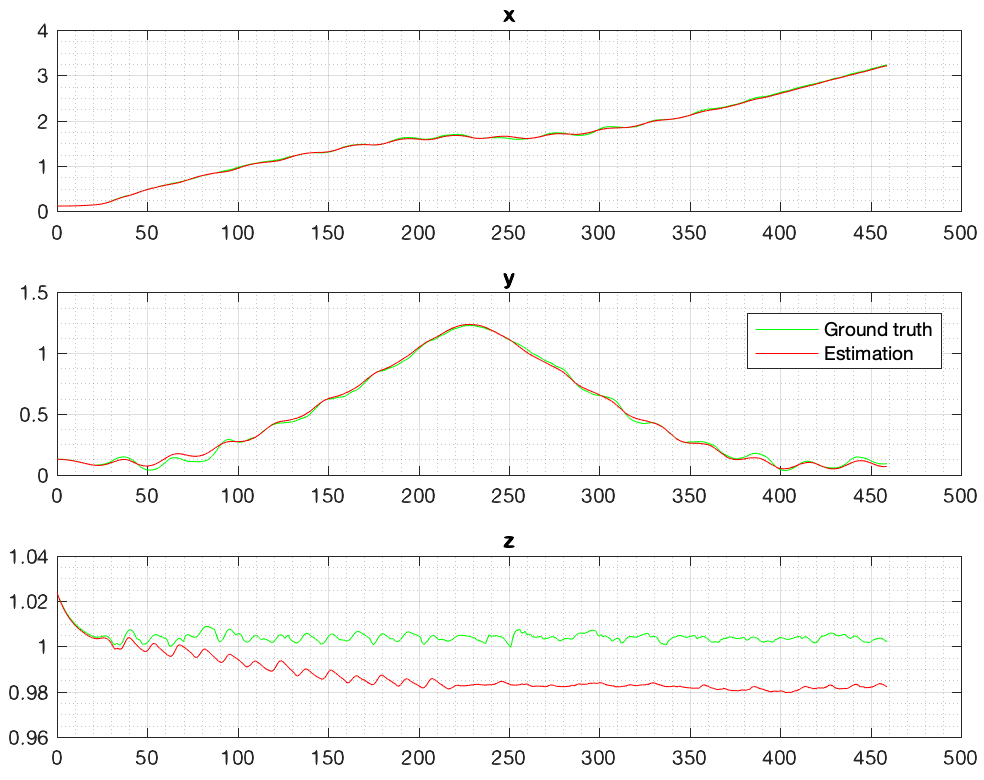
\includegraphics[scale=0.5]{images/trilateration_com.png}
    	\end{figure}
    \end{frame}

    \begin{frame}{MPC Loop CLosure}
    	Given the estimate of the pose of the torso
        $(\bm{\hat{p}}_t, \bm{\hat{o}}_t)^T$,
        it is possible to obtain the estimate of the position of the support foot
        $(\bm{\hat{p}}_s, \bm{\hat{o}}_s)^T$  and of the CoM $(\bm{\hat{p}}_{CoM}, \bm{\hat{o}}_{CoM})^T$  using the kinematics relations.

        The position of the CoM in a rotated
        reference frame of the support foot $\mathcal{F}_{s'}$ which has the $z$-axis
        orthogonal to the floor is:
        \begin{equation*}
            \tensor[^{s'}]{\bm{\hat{p}}}{_{CoM}} = \bm{R}^{T}_{z}(\gamma)(\bm{\hat{p}}_{CoM}-\bm{\hat{p}}_{s})
        \end{equation*}
        This position can be used as a reference signal
        in the MPC in order to generate the gait of the humanoid robot.
    \end{frame}

    \section{Regulation}

    \begin{frame}{Kinematic Model of the Unicycle}
        Brief description:
        \begin{align*}
            \dot{x} &= v \text{cos}(\theta) \\
            \dot{y} &= v \text{sin}(\theta) \\
            \dot{\theta} &= \omega
        \end{align*}
        with $v$ and $\omega$ respectively linear and angular velocity.
    \end{frame}

    \begin{frame}{Proportional Controller}
        \justifying
        Control law:
        \begin{align*}
            v &= k_1 \left\| \bm{p}_g - \bm{\hat{p}}_t \right\| \\
            \omega &= k_2 e_{\theta}
        \end{align*}
        with $e_\theta$ angle between the sagittal vector of the unicycle
        and the vector pointing from the unicycle towards the goal, $k_1 =
        0.18$ and $k_2 = 0.014$. Forcing $v$ and $\omega$ to zero when
        $\left\|\bm{p}_g - \bm{\hat{p}}_t \right\| < 0.25$.
        Desired and final configuration:
        \begin{align*}
            \bm{q}_g &= (-3, 5, \cdot)^T \\
            \bm{q}_f &= (-2.798, 5.090, 0.98\pi)^T \\
            \bm{\hat{q}}_f &= (-2.885, 5.127, 0.979\pi)^T
        \end{align*}
    \end{frame}

    %\begin{frame}{Proportional Controller}
    %    Desired and final configuration:
    %    \begin{align*}
    %        \bm{q}_g &= (-3, 5, \cdot)^T \\
    %        \bm{q}_f &= (-2.798, 5.090, 0.98\pi)^T \\
    %        \bm{\hat{q}}_f &= (-2.885, 5.127, 0.979\pi)^T
    %    \end{align*}
    %\end{frame}

    \begin{frame}{Proportional Controller: x-y Plot}
        \begin{figure}
            \caption{Todo.}
            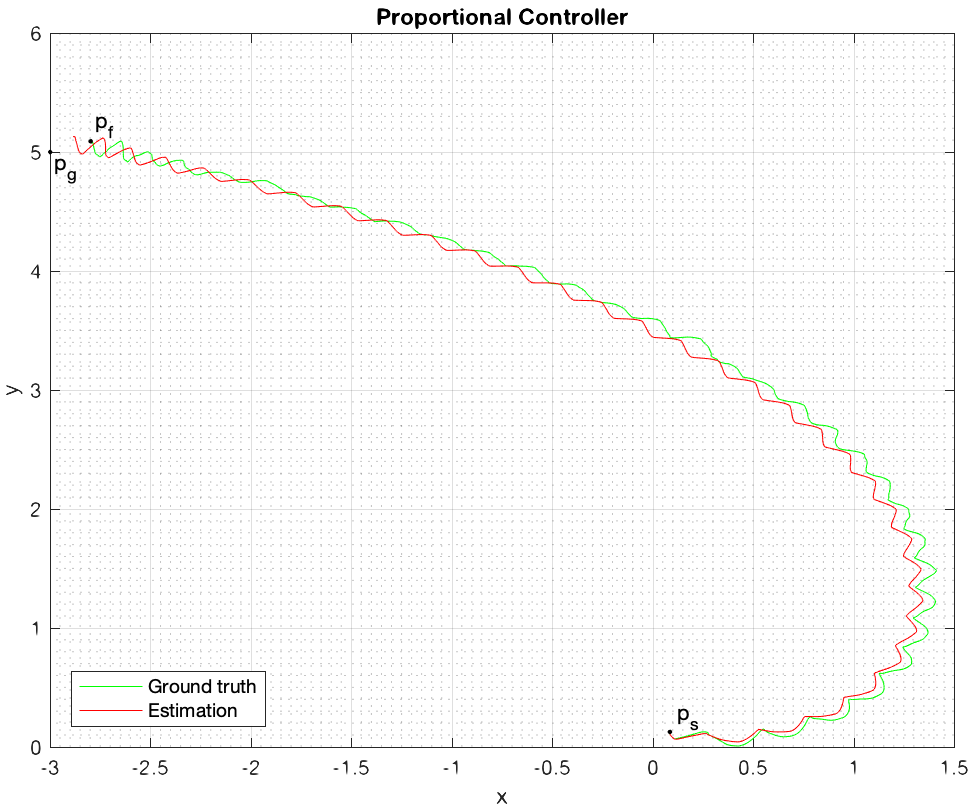
\includegraphics[width=0.75\textwidth]{images/proportional_controller.png}
        \end{figure}
    \end{frame}

    \begin{frame}{Cartesian Regulation}
        \justifying
        Let's express the coordinates of the unicycle in a reference frame
        $\mathcal{F}_g$ fixed at a position $(x_g, y_g)^T$ and
        rotated by $\theta_g$ around $\mathcal{F}_w$:
        \begin{equation*}
            \begin{pmatrix}
                \tensor[^g]{x}{} \\
                \tensor[^g]{y}{} \\
                \tensor[^g]{\theta}{}
            \end{pmatrix}
                =
            \bm{R}_z^T(\theta_g)
            \begin{pmatrix}
                x - x_g \\
                y - y_g \\
                \theta - \theta_g
            \end{pmatrix}
        \end{equation*}
    \end{frame}

    \begin{frame}{Cartesian Regulation}
        \justifying
        Control law:
        \begin{align*}
            v &= -k_1 (\tensor[^g]{x}{} \text{cos}(\tensor[^g]{\theta}{}) + \tensor[^g]{y}{} \text{sin}(\tensor[^g]{\theta}{})) \\
            \omega &=  k_2 (\text{Atan2}(\tensor[^g]{y}{}, \tensor[^g]{x}{}) - \tensor[^g]{\theta}{} + \pi)
        \end{align*}
        with $k_1 = 0.07$ and $k_2 = 0.01$. Forcing $v$ and $\omega$ to zero when
        $\left\|\bm{p}_g - \bm{\hat{p}}_t \right\| < 0.2$.
        Desired and final configuration:
        \begin{align*}
            \bm{q}_g &= (-2, 3.2, \cdot)^T \\
            \bm{q}_f &= (-1.788, 3.105, 1.562\pi)^T \\
            \bm{\hat{q}}_f &= (-1.823, 3.108, 1.562\pi)^T
        \end{align*}
    \end{frame}

    \begin{frame}{Cartesian Regulation: x-y Plot}
        \begin{figure}
            \caption{Todo.}
            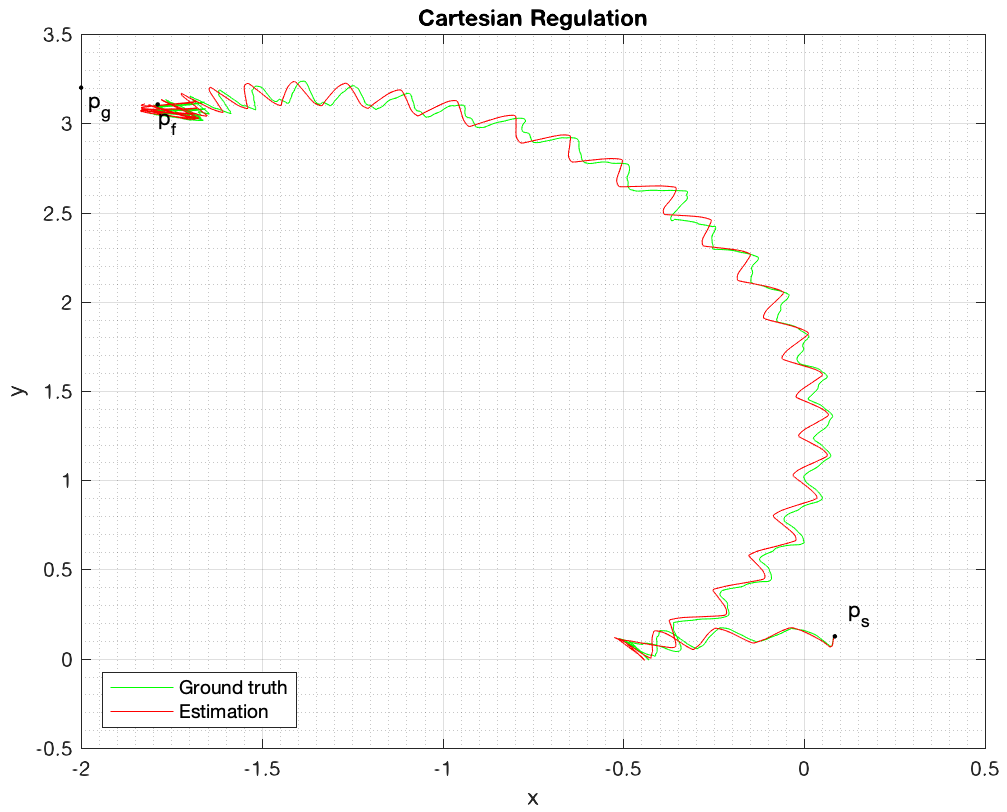
\includegraphics[width=0.75\textwidth]{images/cartesian_regulation.png}
        \end{figure}
    \end{frame}

    \begin{frame}{Kinematic Model of the Unicycle in Polar Coordinates}
        \justifying
        Brief description:
        \begin{align*}
            \dot{\rho}_r &= -v \text{cos}(\gamma_r) \\
            \dot{\gamma}_r &= \frac{\text{sin}(\gamma_r)}{\rho_r}v - \omega \\
            \dot{\delta}_r &= \frac{\text{sin}(\gamma_r)}{\rho_r}v
        \end{align*}
        Polar coordinates can be obtained from the generalized
        coordinates of the unicycle $(x, y, \theta)^T$ by computing:
        \begin{align*}
            \rho_r &= \sqrt{\tensor[^g]{x}{^2} + \tensor[^g]{y}{^2}} \\
            \gamma_r &= \text{Atan2}(\tensor[^g]{y}{}, \tensor[^g]{x}{}) - \tensor[^g]{\theta}{} + \pi \\
            \delta_r &= \gamma_r + \tensor[^g]{\theta}{}
        \end{align*}
    \end{frame}

    \begin{frame}{Posture Regulation}
        \justifying
        Control law:
        \begin{align*}
            v &= k_1 \rho_r \text{cos}(\gamma_r) \\
            w &= k_2 \gamma_r + k_1 \frac{\text{sin}(\gamma_r) \text{cos}(\gamma_r)}{\gamma_r}(\gamma_r + k_3 \delta_r)
        \end{align*}
        with $k_1 = 0.1$, $k_2 = 0.007$ $k_3 = 0.004$. Forcing $v$ and $\omega$ to zero when
        $\rho_r < 0.2$. Desired and final configuration:
        \begin{align*}
            \bm{q}_g &= (-2, 3.2, \pi)^T \\
            \bm{q}_f &= (-1.797, 3.194, 1.024\pi)^T \\
            \bm{\hat{q}}_f &= (-1.824, 3.222, 1.024\pi)^T \\
            \bm{\bar{q}}_f &= (-1.282, 3.424, 0.912\pi)^T
        \end{align*}
    \end{frame}

    \begin{frame}{Posture Regulation: x-y Plot}
        \begin{figure}
            \caption{Todo.}
            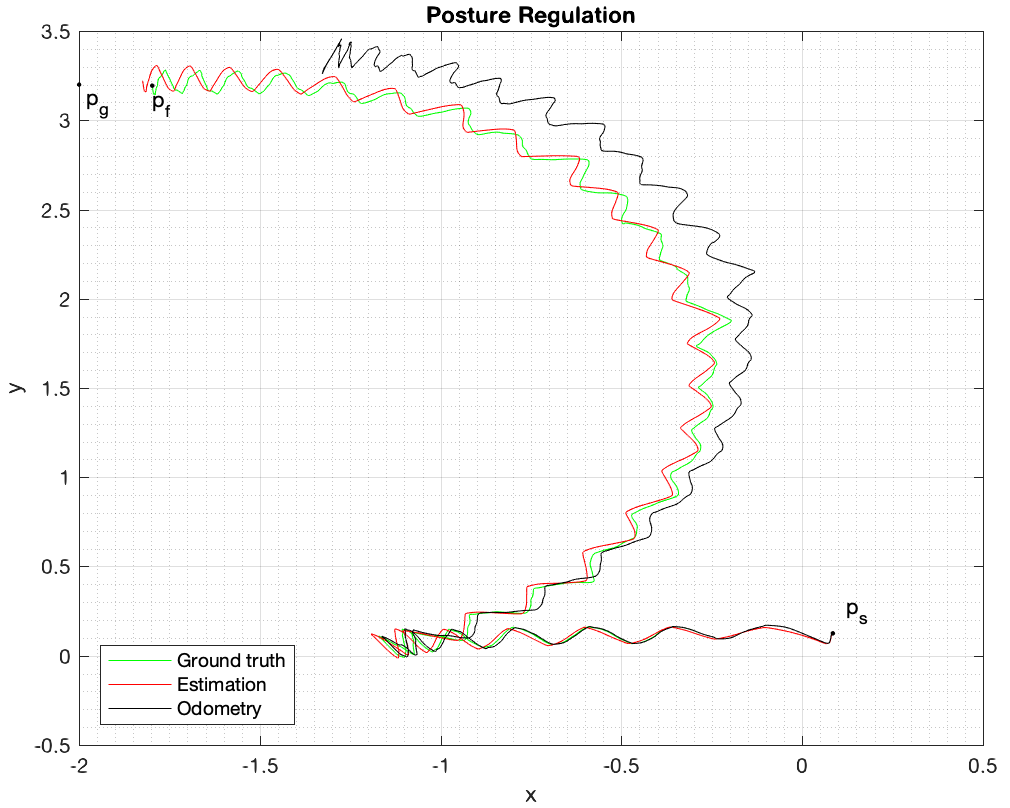
\includegraphics[width=0.75\textwidth]{images/posture_regulation.png}
        \end{figure}
    \end{frame}

    \begin{frame}{Posture Regulation: Yaw Plot}
        \begin{figure}
            \caption{Todo.}
            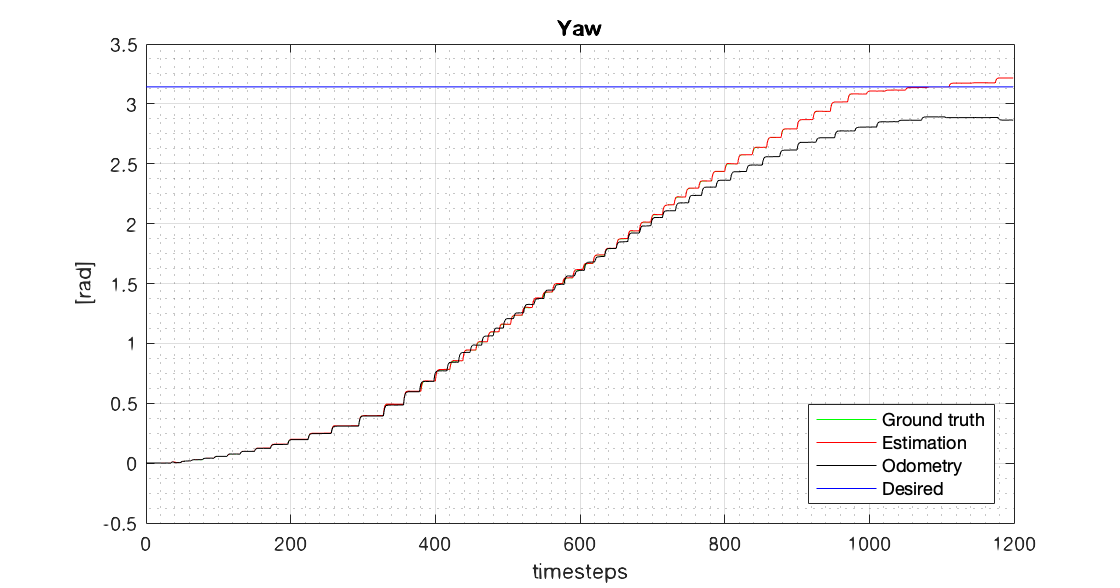
\includegraphics[width=\textwidth]{images/yaw_postureregulation.png}
        \end{figure}
    \end{frame}

    \begin{frame}{Posture Regulation: Velocity Profile Plots}
        \begin{figure}
            \caption{Todo.}
            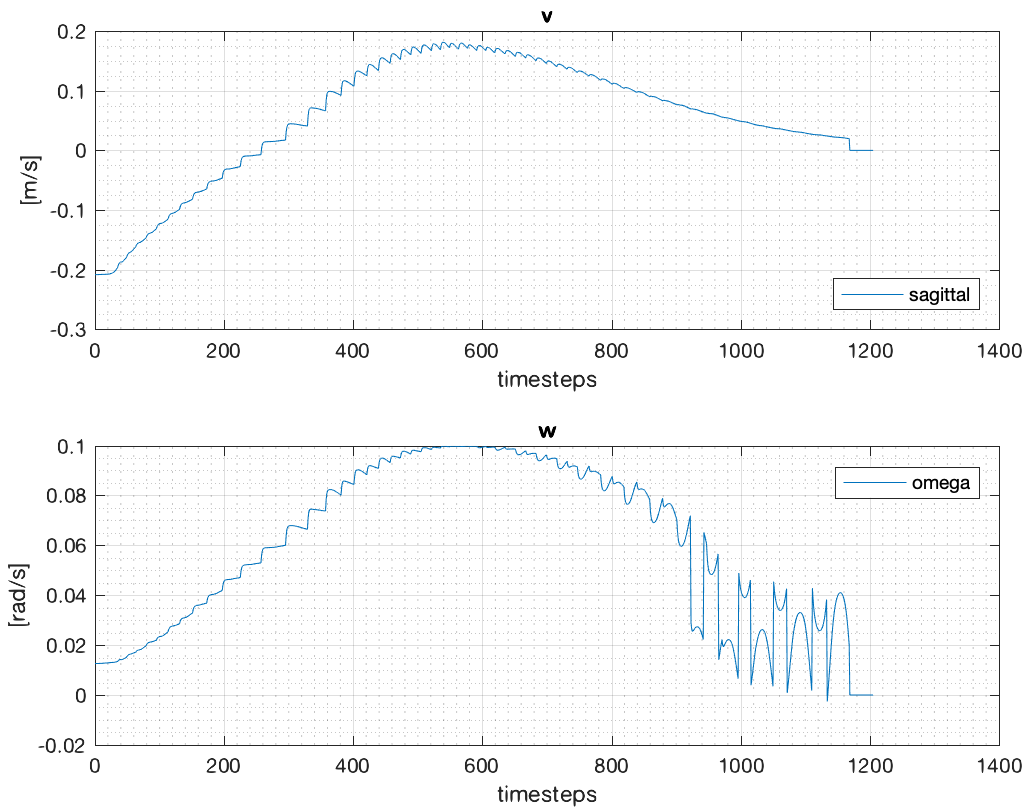
\includegraphics[width=0.8\textwidth]{images/unicycle_velocities.png}
        \end{figure}
    \end{frame}

    \begin{frame}{Conclusion}
        Conclusion.
    \end{frame}

    \begin{frame}[standout]
        Q\&A
    \end{frame}

    \appendix

    \begin{frame}{References}
        \bibliography{bibliography}
        \bibliographystyle{ieeetr}
    \end{frame}

\end{document}
